% !TEX root = document.tex

\chapter{\label{chap:evaluation}Evaluation}

In this chapter, we evaluate the algorithm for traversal fusion in strategic languages developed in the previous chapter. A proof-of-concept implementation that operates on a subset of Stratego has been created. This implementation is run on a synthetic program transformation benchmark that mimics real-world usage, as well as a benchmark simulating a best-case scenario for fusion. The evaluation aims to determine whether traversal fusion works at all in strategic languages, as well as to determine its effect on program runtime and memory usage.

\section{Benchmark Environment}
The benchmarks are run on the following machine:
\begin{itemize}
    \item \textbf{OS:} Windows 11 23H2 (22631.6199)
    \item \textbf{CPU:} Intel Core i7-9750H (6 cores, 2.6 GHz)
    \item \textbf{RAM:} 16 GB DDR4-2666
\end{itemize}

Benchmarks are run in Java using the Java Microbenchmark Harness (JMH). We use it to measure the elapsed program runtime and overall memory usage. In addition, JMH manages, among other things, Java Virtual Machine (JVM) warm-up, repeated runs, and result collection. Finally, a Python script is used to process the results and generate visualizations.

For all benchmarks, JMH has been configured to perform five warm-up runs, after which runtimes stabilize. After that, a series of measured runs is performed (normally ten, unless otherwise mentioned). In the resulting graphs, we use the mean of these ten runs, while the error bars represent one standard deviation.

\section{Benchmark Design}
It is important to design a benchmark that reflects real-world applications of strategic programming languages, because the number of fusion opportunities can differ significantly between different programs. The number of fusion opportunities, of course, directly influences the effectiveness of the traversal fusion optimization. The benchmark created for this evaluation performs several program transformations on a render tree for a custom web design language. This is a relevant real-world use case for strategic programming languages. Furthermore, the benchmark is based on a benchmark used as part of the evaluation for Grafter (the algorithm our solution is also based on), in which it was also selected for its real-world relevance \cite{SakkaSN019}. This also allows for a direct comparison between the effectiveness of our algorithm for strategic programming languages and the algorithm for imperative languages.

In addition to this render tree benchmark, a smaller benchmark simulating a best-case scenario for fusion has also been created. This benchmark consists of a simple binary tree of integers on which two top-down traversals are performed. These traversals can be fully fused into a single top-down traversal.

In the following section, the render tree and the transformations applied to it in the benchmarks will be explained in more detail. The actual Stratego implementation will differ slightly from this explanation in some cases. For example, there are more constructors that contain more fields, and the rewrite rulesets have more definitions. In most cases, these changes were made to work around limitations of the supported subset of Stratego. These implementation details are not relevant for understanding the benchmark and the results.

\subsection{Render Tree and Transformations}
The render tree used in this benchmark is, in essence, an abstract syntax tree representing the structure of a (simple) web page. Pages can have containers that contain elements such as text boxes or images. \autoref{fig:benchmark-render-tree-layout} shows the possible constructors for the render tree and how they relate in more detail. Note that the constructors \texttt{HorizontalContainer} and \texttt{VerticalContainer} are mutually recursive, allowing for complex nested render trees to be created.

The benchmark input size is measured in a number of pages. Every page is an identical sample page that contains each possible type of element (see \autoref{fig:benchmark-render-tree-sample-page}). This sample page is identical to the one used in the Grafter evaluation.

\begin{figure}
\centering
\begin{subfigure}{0.7\textwidth}
\centering
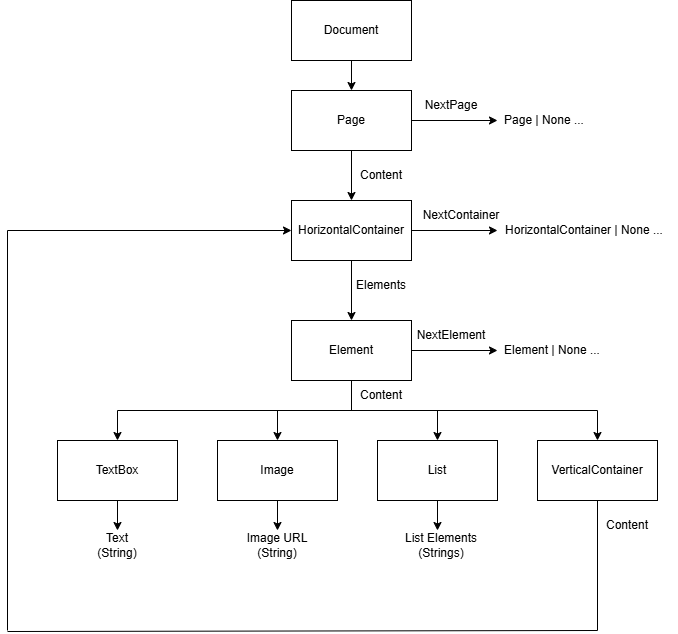
\includegraphics[width=\textwidth]{./img/benchmark-render-tree-layout.png}
\caption{Class layout of the render tree used in the evaluation.}
\label{fig:benchmark-render-tree-layout}
\end{subfigure}

\begin{subfigure}{0.7\textwidth}
\centering
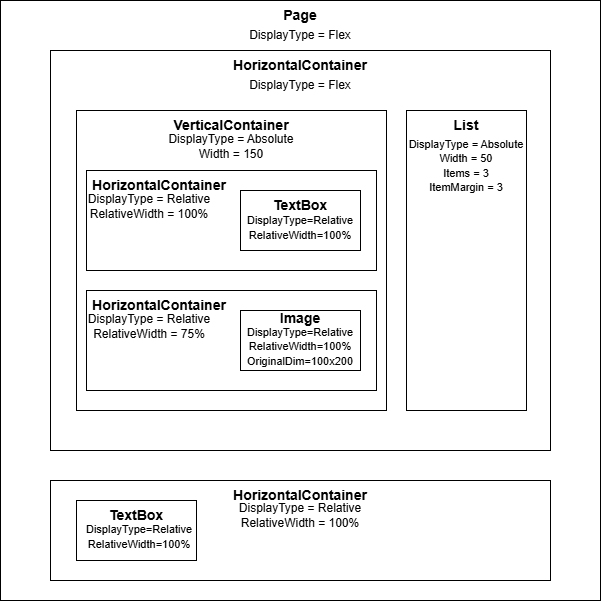
\includegraphics[width=\textwidth]{./img/samplepage.png}
\caption{Sample page used in the render tree benchmark.}
\label{fig:benchmark-render-tree-sample-page}
\end{subfigure}

\caption{Class layout and sample page for the render tree benchmark.}
\label{fig:render-tree-outline}
\end{figure}

Every element contains fields that store properties such as width, height, and position. The purpose of the applied transformations is to compute and fill in these properties for every element. This simulates rendering the web page. In addition, every element stores its display type (flex, relative, or absolute). Elements with different display types interact with their parent and child nodes in different ways, creating complex dependency relations.

In total, five transformations are applied across five consecutive traversals of the render tree:

\begin{enumerate}
    \item Resolve flex width (bottom-up)
    \item Resolve relative width (top-down)
    \item Set font (top-down)
    \item Compute height (bottom-up)
    \item Compute positions (top-down)
\end{enumerate}

The first two traversals compute the widths of every element. Widths for flex elements are computed first, and they have to be computed bottom-up because flex elements expand to fit all their children (and as such their widths depend on the widths of their children). If they were to be computed top-down, there would be no information about the children yet. Then, the widths for relative elements are computed top-down, because the widths of relative elements depend on the widths of their parents.

The third traversal simply takes the font style of the entire document and propagates it down into all children.

Then, the fourth traversal computes the height for every element. A height is computed for every element such as text boxes. Horizontal containers are assigned the maximum computed height of all their children, and the heights of all horizontal containers are summed to compute the height for the page. This also occurs bottom-up.

Finally, the fifth traversal computes the \texttt{x-} and \texttt{y-} positions of every element. The page is assigned position $(0,0)$. Then, a top-down traversal computes all positions by offsetting every element according to all previous widths and heights. For example, if the first element is placed at position $(0,0)$ and has a width and height of $100$, the next element will be placed at position $(100,100)$. If that element has the same width and height, the next element will be placed at $(200,200)$, etc.

\subsection{Measured Properties}
We are interested in measuring three properties of the fused and unfused versions of the benchmarks:
\begin{itemize}
    \item Total number of node visits
    \item Overall program runtime
    \item Overall memory usage
\end{itemize}

The total number of node visits shows whether the algorithm is functional, and whether traversal fusion even is a possible optimization for strategic programming. If the fusion algorithm can effectively fuse the benchmark programs, the number of traversals and therefore the number of times nodes are visited should be reduced.

The overall program runtime and memory usage show whether the fusion optimization is also practically useful. There would be little point in performing this optimization on real-world programs if it does not actually cause a measurable reduction in runtime or memory usage.

\section{Results}
First, we find that it is possible to perform traversal fusion in strategic programming. In the best-case scenario benchmark that achieves full fusion, the number of node visits is reduced by 50\%, as expected. In the render tree benchmark, the total number of node visits is reduced by 41.9\% as a result of traversal fusion. The fusion itself is also interesting: the first and second traversals (computing the width) are fused together into a single traversal, as are the third, fourth, and fifth. The first and second traversal both write to the width field of elements, and one is bottom-up while the other is top-down. Still, it is apparently possible to fuse them. Computing an element's position is done top-down, and is dependent on element height, which is computed bottom-up. Yet, these two things can apparently also be done in a single traversal, even while setting the font style at the same time (which can also influence the height of text boxes).

The original version of the program is much more intuitive to write, and it would not be trivial to design and implement these fused traversals by hand, for the reasons listed above. This shows a clear application of automated traversal fusion.

We have not measured any differences in total memory usage between fused and unfused programs.

\subsection{Performance Impact}
Although traversal fusion is possible in strategic programming, there is one important caveat. At first glance, the fused version of the render tree program seems to achieve a significant mean runtime speedup of approximately 51\% on large enough inputs (there are significant error margins, but the effect is still clearly measurable). On a 1000 page input, the original render tree program has a mean runtime of $\mu=2593$ ms with a standard deviation of $\sigma = 47$ ms. The fused version was measured to have a mean runtime $\mu = 1256$ ms with $\sigma = 64$ ms on the same input.

However, in verifying these results, it became apparent that this speedup was caused almost entirely by the code synthesis, \textbf{regardless} of whether fusion was enabled or not. This is shown in \autoref{fig:bm-rdt}.

\begin{figure}
\centering
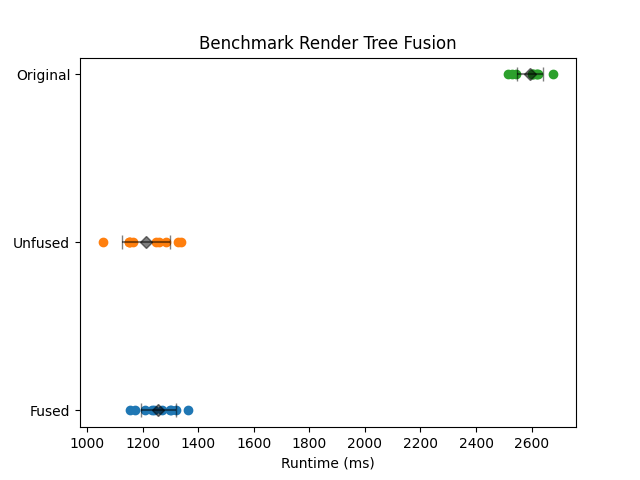
\includegraphics[height=8cm]{./img/rdt_fusion.png}
\caption{Comparison of original, rewritten but unfused, and fused runtimes for the render tree benchmark (n=1000 pages).}
\label{fig:bm-rdt}
\end{figure}

The code generated by the algorithm without applying fusion logically visits the same number of nodes as the input version, but fully accounts for the 51\% speedup. And although it is within the margin of error, it was even measured to be slightly faster than the fused version in this case, with mean runtime $\mu = 1212$ ms and $\sigma = 87$ ms. This means that enabling fusion could very well have no effect at all for this benchmark. This clearly affects the real-world benefit of applying this optimization.

Interestingly, the speedup also does not seem to be affected by the input size (other than the fact that there is a minimum size below which runtimes are too fast to be able to make meaningful measurements). This is not consistent with what would be expected for the traversal fusion optimization, nor is it consistent with the Grafter evaluation, in which larger inputs drastically increase speedup as expected \cite{SakkaSN019}. All of this indicates that the speedup is caused by something else. This is further discussed in \autoref{sec:bm-discussion}.

Although traversal optimization is thus unable to achieve real-world performance improvements for the render tree program, it can provide a measurable performance improvement in the best-case scenario benchmark. \autoref{fig:bm-full} shows that the fused version is significantly faster than both the input program and the version of the program that has gone through code synthesis with fusion disabled. On a binary tree of depth 17 ($2^{17} - 1$ nodes), the original program has a mean runtime of $\mu = 677$ ms with $\sigma = 51$ ms. Code synthesis without fusion achieves a speedup of approximately 16\% ($\mu = 571$ ms, $\sigma = 58$ ms), while fusion achieves a total speedup of 48\% ($\mu = 351$ ms, $\sigma = 44$ ms).\footnote{Two outliers $>1500$ ms have been removed for both the original and unfused versions. The fused version had no significant outliers.}

\begin{figure}
\centering
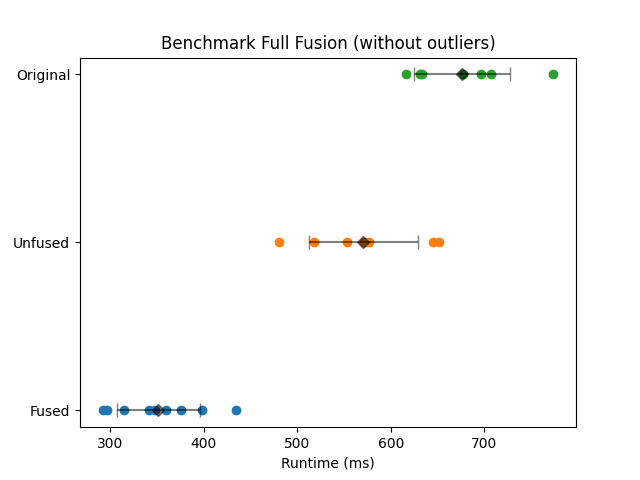
\includegraphics[height=8cm]{./img/full_fusion_no_outliers.png}
\caption{Comparison of original, rewritten but unfused, and fused runtimes for a synthetic benchmark that achieves full fusion (n=$2^{17} - 1$ nodes).}
\label{fig:bm-full}
\end{figure}

\section{Discussion}
\label{sec:bm-discussion}
Traversal optimization performs as expected in the best-case scenario benchmark. In the real-world render tree benchmark, we have seen that synthesizing code without enabling fusion can achieve a significant runtime speedup, while subsequently enabling fusion seems to have little to no further impact. These results require further investigation.

We also discuss the practical applicability of the traversal fusion optimization for strategic programming.

\subsection{Lack of Fusion Speedup}
The fact that traversal fusion significantly reduces the number of node visits in both the render tree and best-case benchmarks means that we also expected to see a significant speedup. The fact that this speedup is present in the best-case scenario benchmark, but not in the render tree benchmark, seems to indicate that traversal fusion introduces some other overhead.

It is not clear what the source of this overhead is, but it is most likely related to one of the following aspects in which the render tree benchmark differs from the best-case scenario benchmark. First, partial fusion requires more complex traversal functions with conditionals compared to unfused or fully fused programs. Simple traversal functions may be easier to optimize, have better interactions with the JVM, or simply perform better for any other reason. Second, the render tree benchmark contains many more node types, constructors, and rewrite rules. It is possible that this causes additional overhead, possibly in combination with any overhead already caused by partial fusion. We have not been able to identify the actual source of the overhead, and it is possible that there is another cause.

Another interesting theory is that there is another source of overhead unrelated to the traversals. For example, this could be the application of the rewrite rules themselves. Traversal fusion, as we have seen, cannot change the number of applications of rewrite rules. This source of overhead could be so large that the total traversal time is simply too small in comparison for traversal fusion to have a measurable effect. For example, suppose that there are 1000 traversal calls and 1000 rewrite rule applications, and traversal fusion reduces this to 500 traversal calls and 1000 rewrite rule applications. If the rewrite rules dominate the total runtime (e.g. they take $1$ ms each, while the traversal calls take $1$ ns each), we would expect no significant runtime impact due to traversal fusion.

To verify whether this is at least a plausible theory, we have created an alternate version of the render tree benchmark in which every traversal call includes a busy-wait of a certain amount of time. We then compare the version that has gone through code synthesis with fusion disabled with the fused version. The results of this comparison are shown in \autoref{fig:bm-add-time}. Indeed, artificially increasing the amount of time that the traversal calls take relative to the rest of the program increases the benefit of traversal optimization. Without additional traversal time, the versions have almost equal performance. At $5$ $\mu$s additional time, the fused version is 23\% faster, and at $20$ $\mu$s the fused version is approximately 31\% faster.

\begin{figure}
\centering
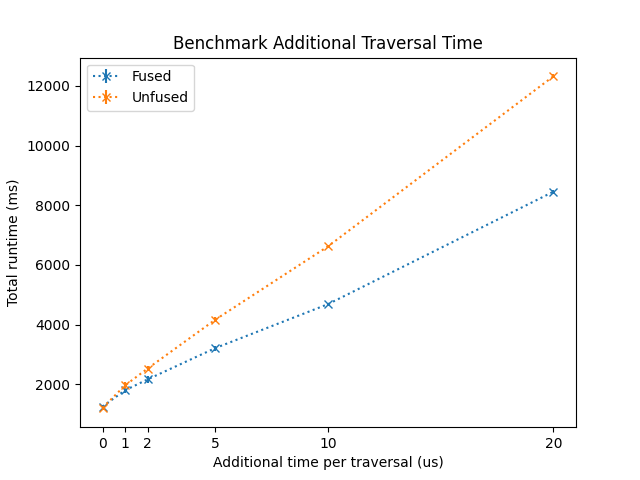
\includegraphics[height=8cm]{./img/add_traversal_time_full.png}
\caption{Comparison of unfused and fused mean runtimes for the render tree benchmark, with increasing additional traversal time (n=1000 pages).}
\label{fig:bm-add-time}
\end{figure}

\subsection{Code Synthesis Speedup}
Our theories to explain the lack of speedup due to traversal fusion do not explain the speedup that occurs after code synthesis without fusion. Although it is out of scope for this thesis to explore this speedup, it being unrelated to traversal fusion, it is certainly interesting. The most likely cause is an unexpected JVM interaction or some other Stratego-specific effect. Still, it may be interesting to investigate this speedup in the context of traversal fusion in the future, as we cannot rule out that it is related to the lack of speedup we have seen for traversal fusion.

\subsection{Further Discussion}
Although we can conclude that traversal optimization is possible in strategic programming, the results of this evaluation raise concerns about practical applicability.

For compiler designers, implementing additional optimizations means investing time, an increase in compiler complexity, and an increase in compiler overhead. As such, implementing an optimization is always a trade-off, and this only makes sense if the optimization provides a significant benefit relative to the cost of implementing it.

The lack of speedup in the render tree benchmark indicates that there is little point in performing fusion for such a program in a real-world scenario. The traversal fusion optimization itself is also relatively complex, and its performance scales poorly with input program size (because it finds all possible fusions). The complexity of the optimization is certainly an important factor: it increases the chances of compiler bugs, which could lead to potentially incorrectly compiled code. Compiler bugs are notoriously hard to deal with for programmers and could carry significant consequences if not caught. If there is indeed little benefit to performing the optimization, it would be hard to conclude that the trade-off favors implementing the traversal fusion optimization in this case.

On the other hand, we have identified two cases in which fusion does provide a significant speedup (namely, when performing full fusion on a simpler program, and when artificially increasing traversal time). These benchmarks are further removed from real-world applications, but in theory these situations certainly could occur. In addition, we have not identified situations in which fusion creates a slower program. For a programmer writing programs in a strategic language, there is little cost in performing the optimization (other than increased compiler runtime), meaning even a relatively small chance of increased performance could certainly be worth it.

In any case, we would argue that it is at least possible in theory that the issue of fusion not providing a speedup could be solved. If it can, this would certainly shift the trade-off to be in favor of implementing it, because the performance increase can be very significant. If this issue cannot be solved, it could be worth at least investigating whether there exists a test that can be performed quickly to predict whether fusion could provide a benefit for a certain program.

We feel that it is fair to conclude that, although there are valid concerns about the practical applicability that would prevent this optimization from being implemented right now, it is too early to give up on it entirely in strategic programming.

\section{Validity}
There are two main factors that can impact the validity of this evaluation.

First, a significant factor is the generalizability of these results. We aim to assess the effect of the traversal fusion optimization on strategic programs in general. To do this, we evaluate an implementation on a subset of one strategic programming language, Stratego. On top of that, the render tree benchmark is based on a domain in which strategic programming languages are normally used, but may not be fully representative (and it has also been selected to fit within the supported subset of Stratego). We do note, in defense of this approach, that:
\begin{itemize}
    \item It is true that the performance impact may differ depending on many factors, but the core result of whether traversal fusion works at all is easily generalizable to all strategic languages. We have shown that for a large program, similar to real-world applications, the algorithm can correctly identify fusion opportunities and synthesize fused traversal code.
    \item Although the render tree benchmark has been carefully selected to be representative, the performance of the traversal fusion optimization may still differ significantly between programs. This depends mainly on the number of fusion opportunities available for that program. That does mean that the optimization may be more effective for certain types of programs than it is for others. However, this is true for for most optimizations. Although of course a simplification, we could say that traversal fusion suffers from a lack of fusion opportunities in the same way that an optimization such as loop unrolling suffers from a lack of loops to unroll. In general, the optimization may still be viable.
\end{itemize}

Second, the goal of measuring the impact of the traversal fusion optimization can be adequately achieved by measuring the program runtime. However, this is the overall program runtime, which is subject to significant variance. We have noticed that Stratego programs always seem to have a significant variance in runtime. On top of that, the overall program runtime includes operations such as reading the input data. Although these operations are identical for each benchmark that is compared, they may introduce additional variance in the data. On the other hand, variance in the program runtime is also controlled by including warm-up runs through JMH. Still, variance remains a significant factor, and four significant outliers had to be excluded from the best-case scenario benchmark.